\chapter{Cloud Computing} % (fold)
\label{cha:Cloud Computing}

\section{Was ist Cloud Computing?} % (fold)
\label{sec:Was ist Cloud Computing}

„Cloud-Computing, häufig auch als „die Cloud“ bezeichnet, ist die Bereitstellung von IT-Ressourcen – von Anwendungen bis zu Rechenzentren – bei Bedarf über das Internet auf der Basis nutzungsabhängiger Gebühren.“ \footcite[][]{o.V..2020} \\
Abbildung \ref{abb:ElementeCloudComputing} soll hier den Aufbau und die Elemente des Cloud Computing bild- und schemenhaft darstellen.

\begin{figure}[htb]
	\centering
	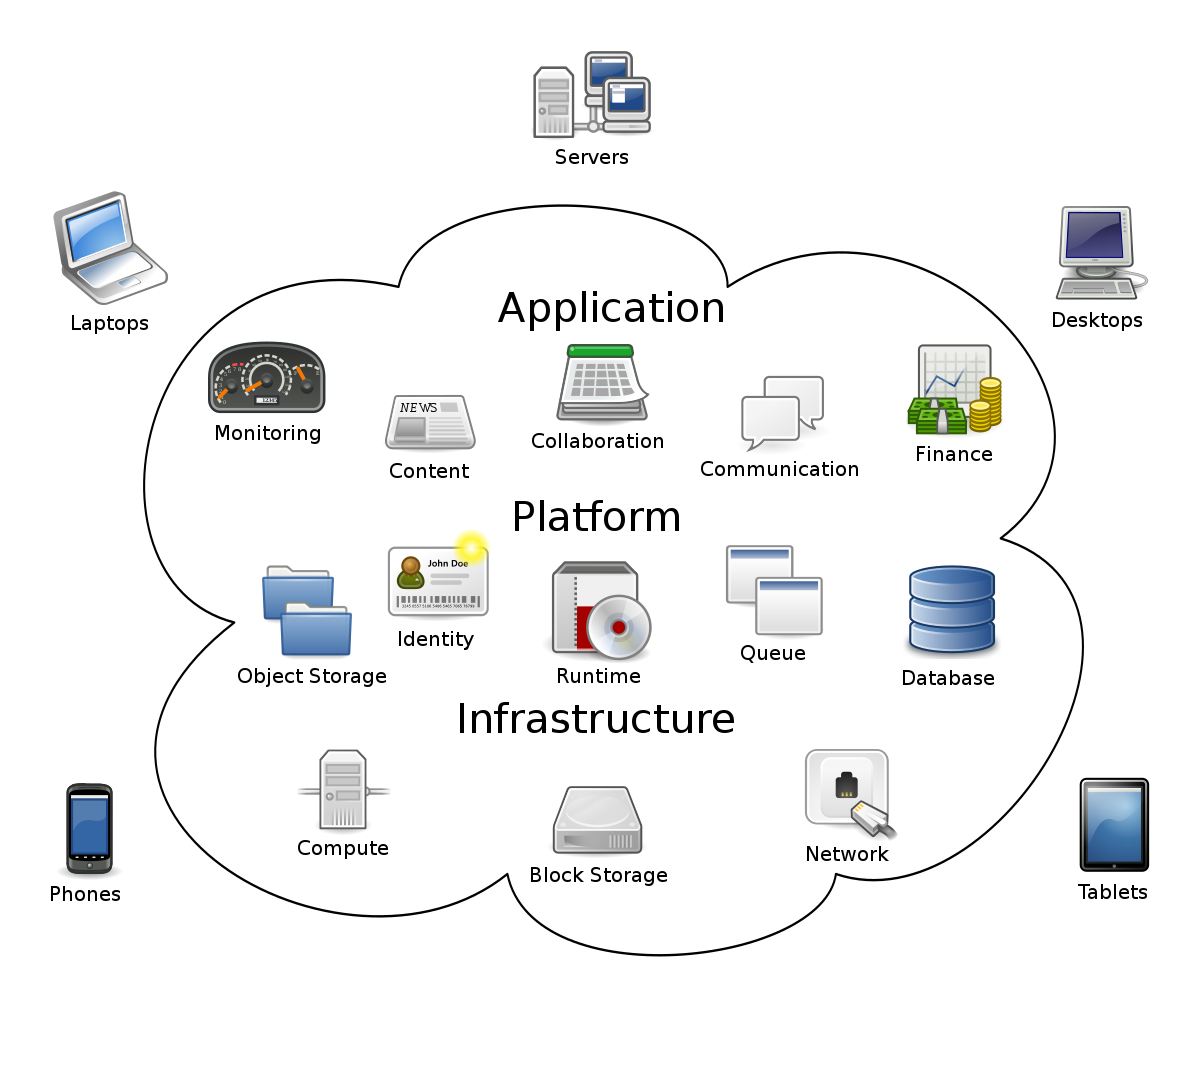
\includegraphics[width=5cm]{graphics/CloudComputing.png}
	\caption[Elemente des Cloud Computing]{Elemente des Cloud Computing \footnotemark}
	\label{abb:ElementeCloudComputing}
\end{figure}
\footnotetext{Entnommen aus: \cite{o.V..2022}}

Das National Institute of Standards and Technology(NIST) definiert zudem 5 Charakteristiken, die Cloud Computing besitzt. \footcite[Vgl.][auch im Folgenden]{Mell.2011}

\begin{description}
	\item \emph{On-demand self-service.} Der Nutzer kann eigenständig und ohne menschliche Interaktion Leistungen, wie Serverzeit und Netzwerkspeicher bereitstellen lassen.
	\item \emph{Broad network access.} Die Leistungen sind im Netzwerk und standardisiert erreichbar und unterstützen die Verwendung durch heterogene Geräte, wie Smartphones, Tablets oder Laptops.
	\item \emph{Ressource pooling.} Die Computerressourcen des Anbieters werden zusammengefasst, um mehrere Nutzer nach dem Mehrmandantenprinzip bedarfsgerecht bedienen zu können. Damit einhergehend hat der Nutzer in der Regel keine Kontroller darüber, mit welchen Computerressourcen die Leistung erbracht wird (z. B. auf welchem Server oder mit welcher Datenbank).
	\item \emph{Rapid elasticity.} Die Leistung kann elastisch bereitgestellt und freigegeben werden, um bedarfsgerecht, in manchen Fällen automatisch, hoch und runter skalieren zu können. Aus Sicht des Nutzers scheinen die verfügbaren Computerressourcen unbegrenzt und Leistungen können jederzeit in beliebiger Höhe angepasst werden.
	\item \emph{Measured service.} Cloud-Systeme steuern und optimieren Computerressourcen anhand von messbaren Zahlen, die, abhängig von der jeweiligen Leistung, erhoben werden wie etwa Speichern Bandbreite oder aktive Benutzerkonten. Die Nutzung der Leistung kann überwach, gesteuert und alt Bericht bereitgestellt werden, um die Transparenz für den Nutzer wie auch den Anbieter gewährleisten zu können.
\end{description}

% section Was ist Cloud Computing (end)

\section{Die Formen des Cloud Computing} % (fold)
\label{sec:Die Formen des Cloud Computing}

Cloud Computing wird in drei wesentliche Formen unterteilt. Die Private Cloud, die Public Cloud und die Hybrid Cloud.
\begin{description}
	\item \emph{Private Cloud} bedeutet, dass eine Infrastruktur für ein einziges Unternehmen, entweder vom Unternehmen selber, oder von einem externen Provider betrieben wird.
	\item \emph{Public Cloud} bedeutet, dass unabhängige Unternehmen IT-Ressourcen zur Verfügung stellen, die von mehreren verschiedenen Unternehmen genutzt werden können, ohne selbst in Hardware, Software oder Infrastruktur investieren zu müssen.
	\item \emph{Hybrid Cloud} basiert auf der Private Cloud und wird häufig verwendet um eine Private Cloud durch Workload-Managment auf Rechenzentren, Private Clouds und Public Clouds aus zu weiten.
\end{description}

% section Die Formen des Cloud ComputingDie Formen des Cloud Computing (end)

\section{Clouddienste} % (fold)
\label{sec:Clouddienste}

Des Weiteren werden verschiedene Clouddienste unterschieden. Diese sind in Abbildung \ref{abb:PizzaModel} am Beispiel einer Pizza bildlich dargestellt und im Folgenden erklärt. \footcite[][]{Mell.2011}

\begin{figure}[htb]
	\centering
	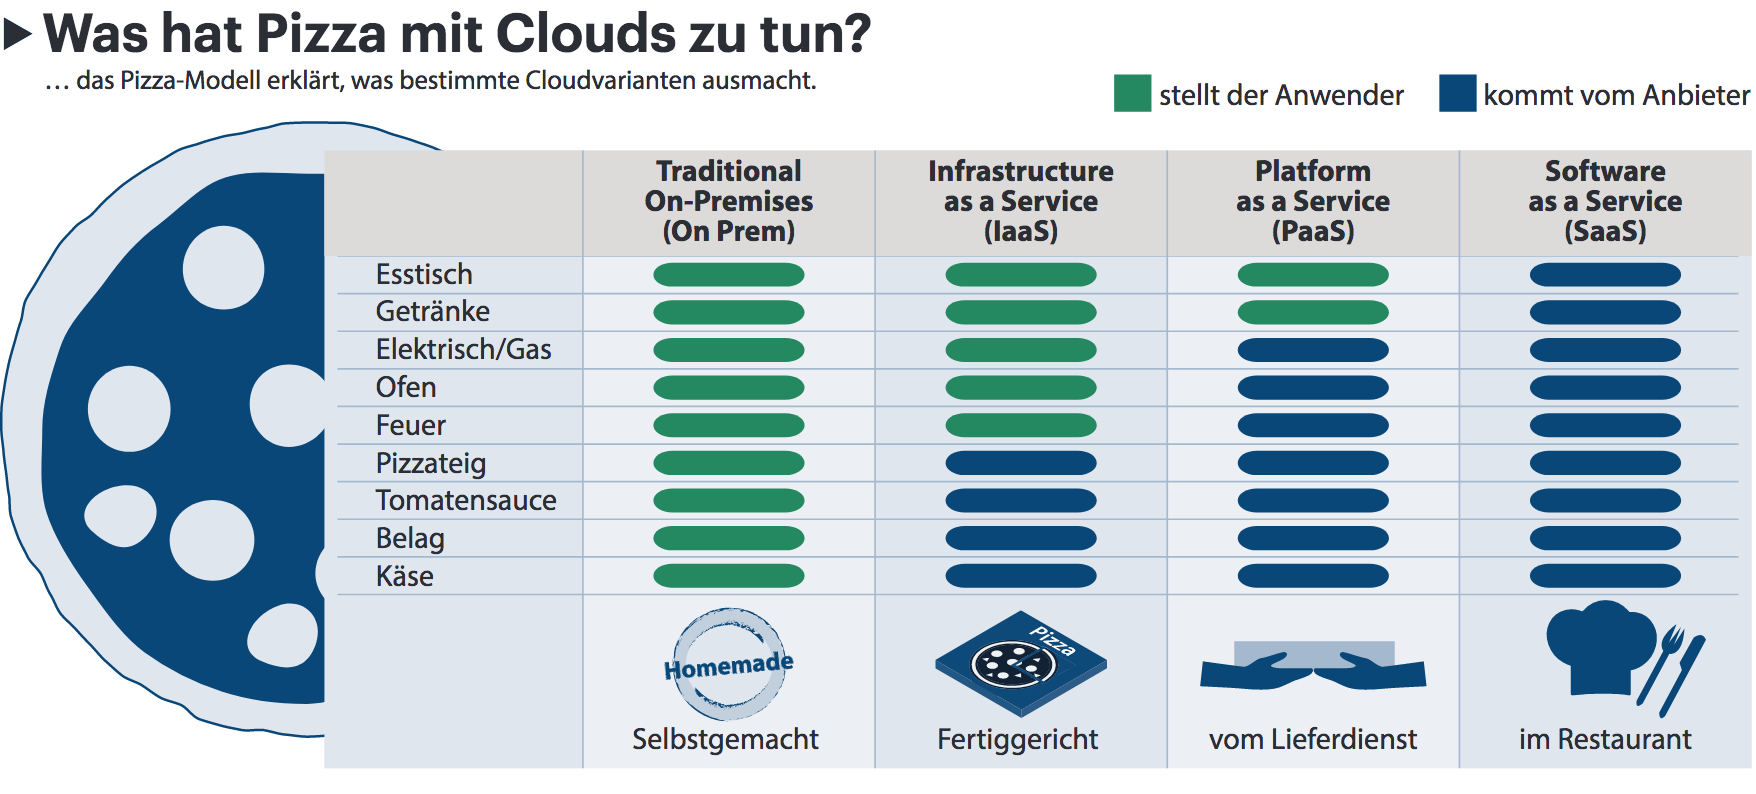
\includegraphics[width=12cm]{graphics/PizzaModel.png}
  \caption[Clouddienste im Pizza-Modell]{Clouddienste im Pizza-Modell \footnotemark}
	\label{abb:PizzaModel}
\end{figure}
\footnotetext{Entnommen aus: \cite{Link.2020}}

\begin{description}
  \item \emph{On Premises (On Prem).} Als On Premises wird die traditionelle, also nicht Cloud-basierte Lösung bezeichnet. Grundsätzlich kann auch bei Cloud-basierten Nutzungsmodellen von „Off Premises“ gesprochen werden.
  \item \emph{Infrastructure as a Service (IaaS).} Der Cloud-Provider bietet Zugang zu virtualisierten Rechnern einschließlich ganzer Betriebssysteme und Speichersysteme.
  \item \emph{Platform as a Service (PaaS).} Hier bietet der Cloud-Provider Zugang zu ganzen Programmierumgebungen zur Entwicklung von Anwendungen an.
  \item \emph{Software as a Service (SaaS).} Bei diesem Clouddienst bietet der Cloud-Provider Zugang zu den Anwendungsprogrammen direkt.
\end{description}

% section Clouddienste (end)

% chapter Cloud Computing (end)
